\documentclass{article}\usepackage[]{graphicx}\usepackage[]{color}
%% maxwidth is the original width if it is less than linewidth
%% otherwise use linewidth (to make sure the graphics do not exceed the margin)
\makeatletter
\def\maxwidth{ %
  \ifdim\Gin@nat@width>\linewidth
    \linewidth
  \else
    \Gin@nat@width
  \fi
}
\makeatother

\definecolor{fgcolor}{rgb}{0.345, 0.345, 0.345}
\newcommand{\hlnum}[1]{\textcolor[rgb]{0.686,0.059,0.569}{#1}}%
\newcommand{\hlstr}[1]{\textcolor[rgb]{0.192,0.494,0.8}{#1}}%
\newcommand{\hlcom}[1]{\textcolor[rgb]{0.678,0.584,0.686}{\textit{#1}}}%
\newcommand{\hlopt}[1]{\textcolor[rgb]{0,0,0}{#1}}%
\newcommand{\hlstd}[1]{\textcolor[rgb]{0.345,0.345,0.345}{#1}}%
\newcommand{\hlkwa}[1]{\textcolor[rgb]{0.161,0.373,0.58}{\textbf{#1}}}%
\newcommand{\hlkwb}[1]{\textcolor[rgb]{0.69,0.353,0.396}{#1}}%
\newcommand{\hlkwc}[1]{\textcolor[rgb]{0.333,0.667,0.333}{#1}}%
\newcommand{\hlkwd}[1]{\textcolor[rgb]{0.737,0.353,0.396}{\textbf{#1}}}%

\usepackage{framed}
\makeatletter
\newenvironment{kframe}{%
 \def\at@end@of@kframe{}%
 \ifinner\ifhmode%
  \def\at@end@of@kframe{\end{minipage}}%
  \begin{minipage}{\columnwidth}%
 \fi\fi%
 \def\FrameCommand##1{\hskip\@totalleftmargin \hskip-\fboxsep
 \colorbox{shadecolor}{##1}\hskip-\fboxsep
     % There is no \\@totalrightmargin, so:
     \hskip-\linewidth \hskip-\@totalleftmargin \hskip\columnwidth}%
 \MakeFramed {\advance\hsize-\width
   \@totalleftmargin\z@ \linewidth\hsize
   \@setminipage}}%
 {\par\unskip\endMakeFramed%
 \at@end@of@kframe}
\makeatother

\definecolor{shadecolor}{rgb}{.97, .97, .97}
\definecolor{messagecolor}{rgb}{0, 0, 0}
\definecolor{warningcolor}{rgb}{1, 0, 1}
\definecolor{errorcolor}{rgb}{1, 0, 0}
\newenvironment{knitrout}{}{} % an empty environment to be redefined in TeX

\usepackage{alltt}
\usepackage{alltt}
\usepackage{amsmath}
\usepackage[sc]{mathpazo}
\usepackage[T1]{fontenc}
\usepackage{geometry}
\geometry{verbose,tmargin=2.5cm,bmargin=2.5cm,lmargin=2.5cm,rmargin=2.5cm}
\setcounter{secnumdepth}{2}
\setcounter{tocdepth}{2}
\usepackage{url}
\usepackage[unicode=true,pdfusetitle,
 bookmarks=true,bookmarksnumbered=true,bookmarksopen=true,bookmarksopenlevel=2,
 breaklinks=false,pdfborder={0 0 1},backref=false,colorlinks=false]
 {hyperref}
\hypersetup{
 pdfstartview={XYZ null null 1}}
 
\title{Some variations on Figure 1 b)} 
 
\usepackage{breakurl}
\IfFileExists{upquote.sty}{\usepackage{upquote}}{}
\begin{document}
\maketitle
%\SweaveOpts{concordance=TRUE}



%Load the necessary libraries, source the file with the R functions:


Will use the same theme throughout, so just declare this variable:

  

\section{AR(1) correlation matrices}

These results are for the $I=2, p\ge 2$ autoregressive case with AR(1) with equal within-study variances,
so the parameters we vary are: $r, \rho_1, \rho_2, p$. 
We save the relative efficiencies for only one of coefficients, as they are all equal.
We consider $\rho_1 = 0$.




The following results are for the $I=20, p\ge 2$ AR(1) case with equal within-study variances
and $S_i^2 \equiv S^2, \rho_i = \frac{\rho(i-1)}{I}$, so the parameters we vary are $\rho, p$.
We save the relative efficiencies for only one of coefficients, as they are all equal.





\section{Block diagonal correlation matrices}

These results are for the $I=2, p\ge 2$ case with block diagonal matrices with block size of 5, compound symmetry
within the blocks, so the parameters we vary are: $r, \rho_1, \rho_2, p$. 
We save the relative efficiencies for only one of coefficients, as they are all equal.
We consider $\rho_1 = 0$.




The following results are for the $I=20, p\ge 2$ 
case with block diagonal matrices with block size of 5, compound symmetry
within the blocks, with equal within-study variances
and $S_i^2 \equiv S^2, \rho_i = \frac{\rho(i-1)}{I}$, so the parameters we vary are $\rho, p$.
We save the relative efficiencies for only one of coefficients, as they are all equal.





\section{Put all four panels together}

\begin{knitrout}
\definecolor{shadecolor}{rgb}{0.969, 0.969, 0.969}\color{fgcolor}\begin{kframe}


{\ttfamily\noindent\itshape\color{messagecolor}{\#\# Loading required package: grid}}\end{kframe}

{\centering 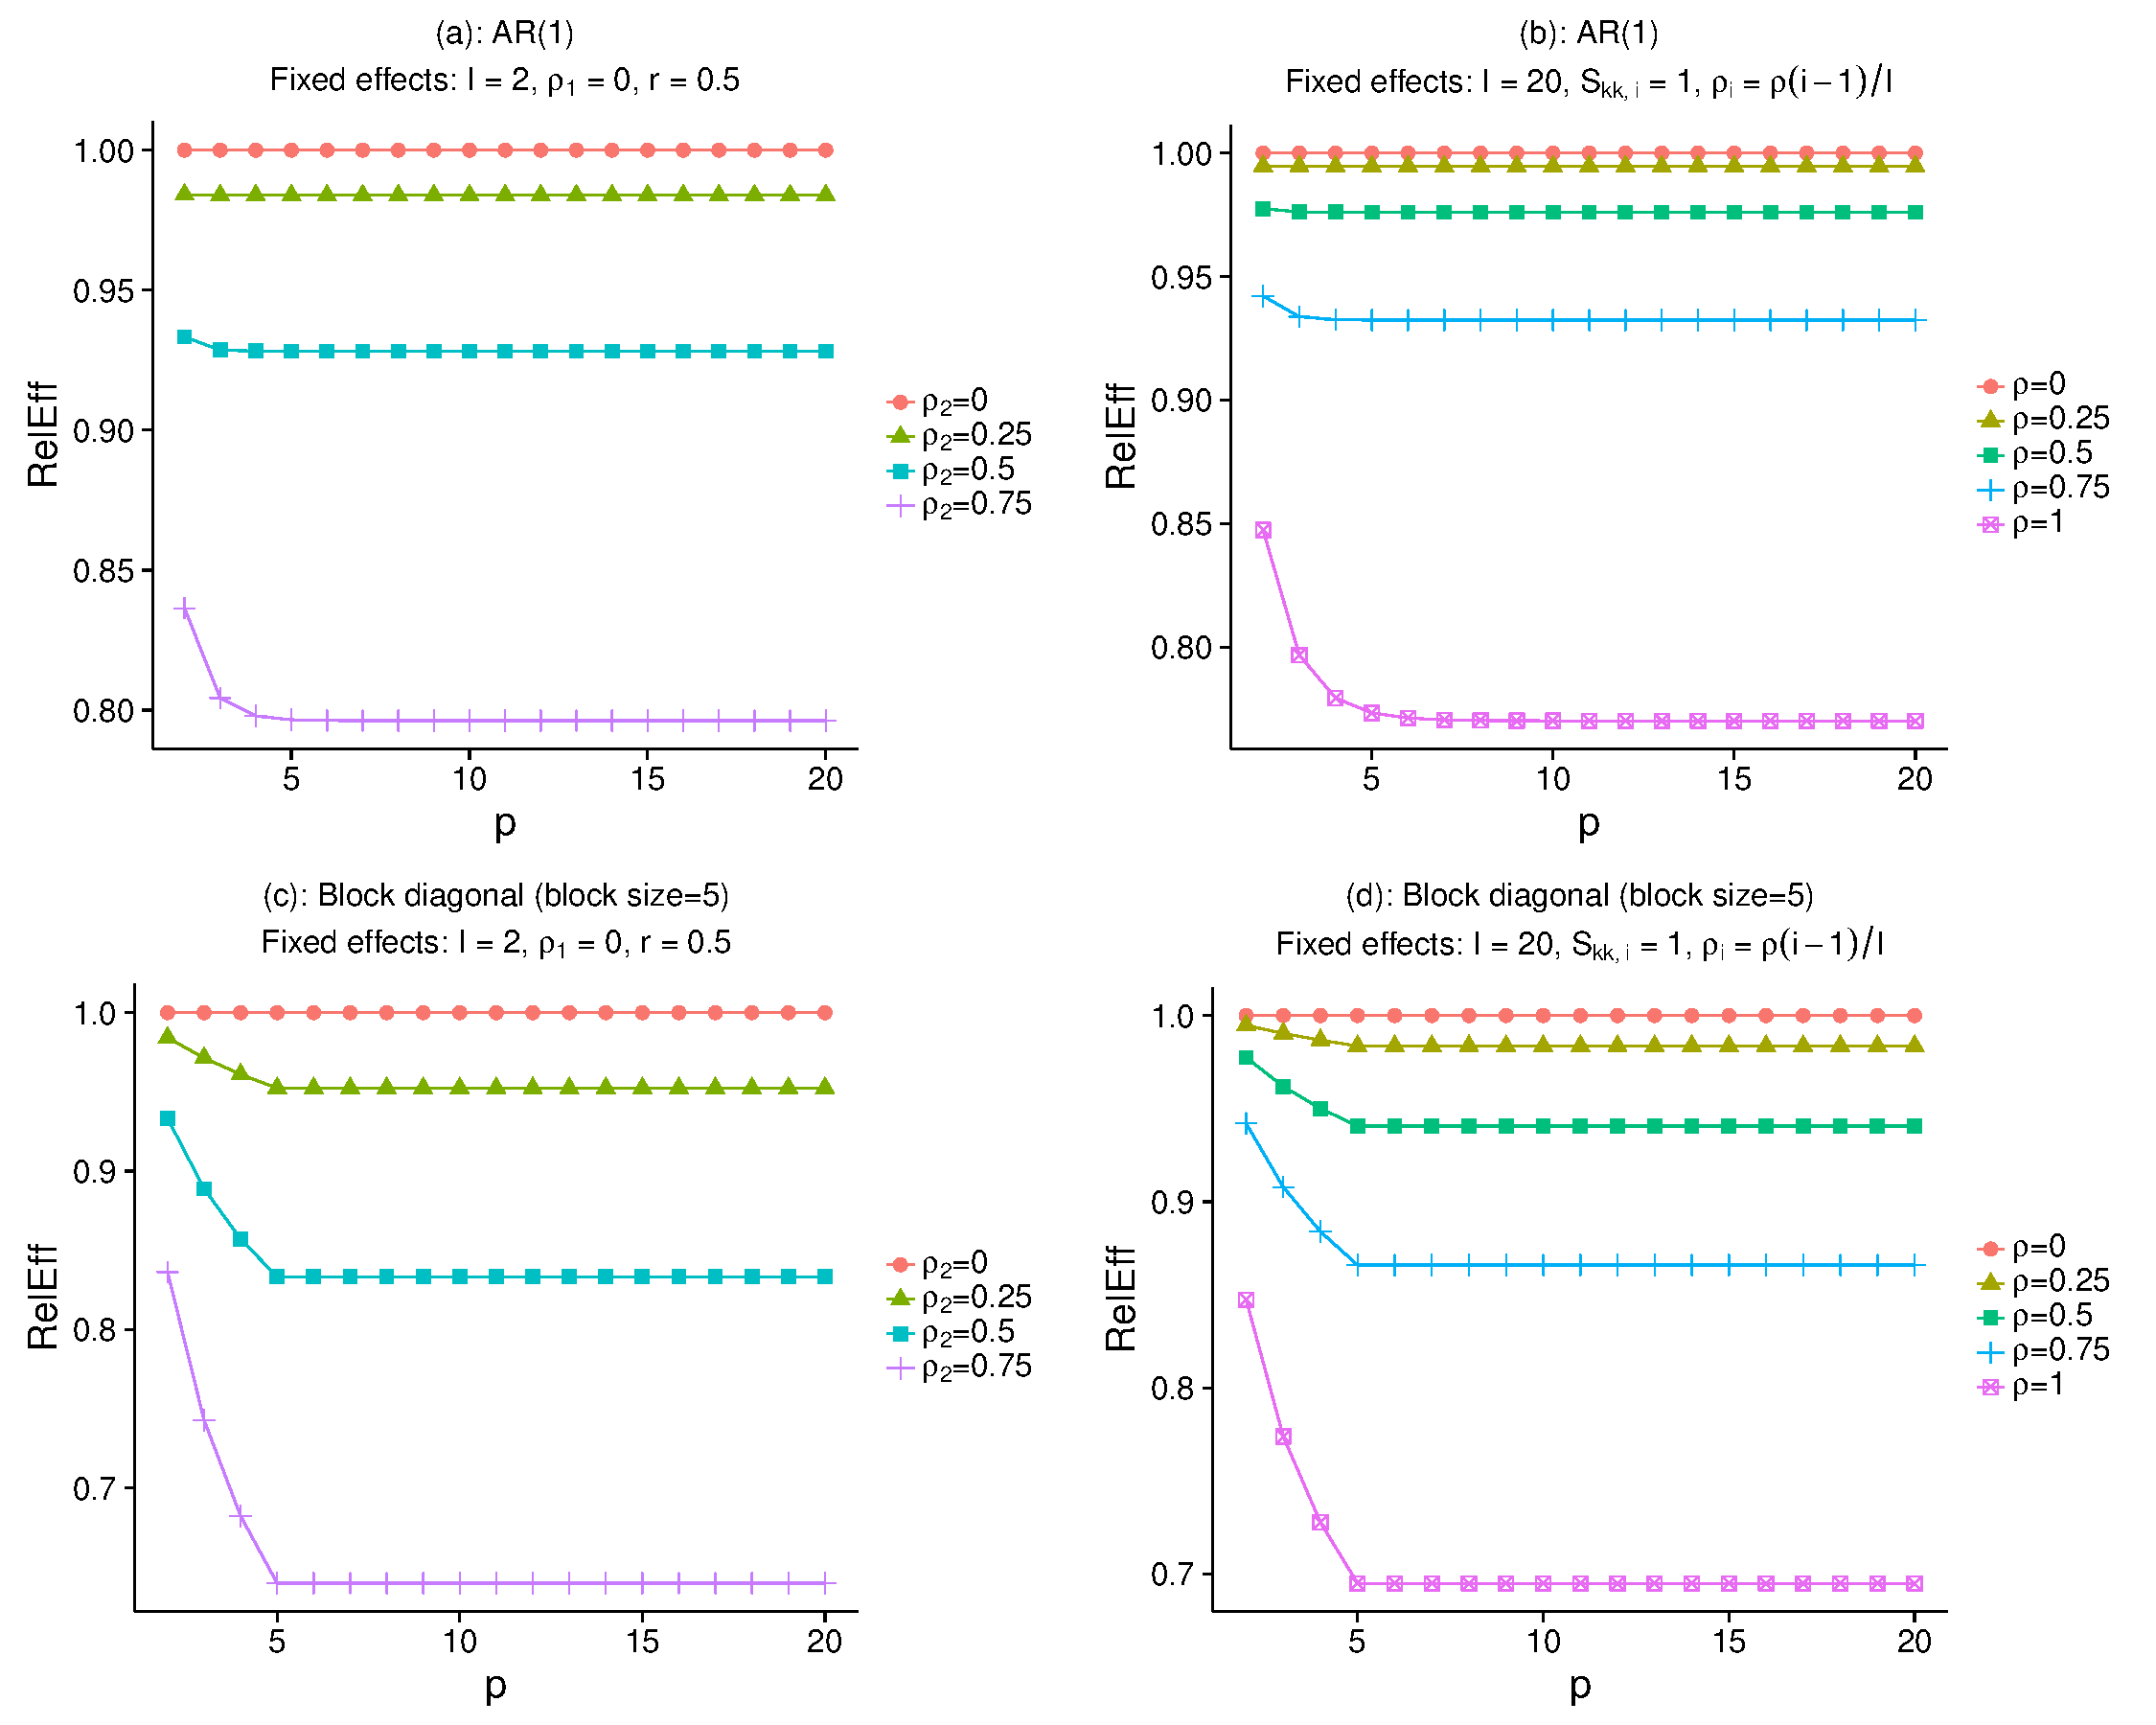
\includegraphics[width=\maxwidth]{figures/Figure_S7_panels_abcd-1} 

}



\end{knitrout}


\end{document}










